\section{Catastrophic Forgetting Dynamics and Benchmarks}

Having established the lifecycle and paradigms of continual learning, this section examines \emph{why} catastrophic forgetting occurs and \emph{how} it is measured. The findings here motivate a central design commitment of this work: because parametric tuning forgets as a matter of principle, volatile factual knowledge is better externalized into a non-parametric memory.

\subsection{The Inverse Linear Law of Forgetting}
Kalajdzievski \parencite{kalajdzievski2024scalinglawsforgettingfinetuning} establishes an \textbf{Inverse Linear Law}: the degree of forgetting $L_f$ scales linearly with the fine-tuning loss $L_{ft}$, meaning that the more thoroughly a model learns a new task, the more it forgets prior knowledge. A critical corollary is that common practitioner heuristics---reducing the LoRA rank or applying early stopping---do not prevent forgetting; they merely reduce how well the new task is learned. Forgetting is further shown to erode safety guardrails, as LoRA fine-tuning measurably degrades refusal behavior on adversarial prompts. This law implies that any approach that integrates knowledge \emph{into the weights} pays a proportional forgetting cost, which a frozen-backbone design avoids entirely.

\subsection{Loss Landscape Geometry and Optimizer Remedies}
Li et al. \parencite{li2024revisitingcatastrophicforgettinglarge} attribute forgetting to the geometry of the loss landscape: fine-tuning on out-of-distribution data drives weights into \emph{sharp} minima where small parameter shifts cause large loss spikes on prior tasks. Sharpness-Aware Minimization (SAM) instead locates \emph{flat} minima that are robust to such shifts, and operates orthogonally to data replay (their effects compound, with reported gains of up to $+3.02\%$ in retention). Figure~\ref{fig:loss_landscape} contrasts the two regimes. Complementarily, Luo et al. \parencite{luo2025empiricalstudycatastrophicforgetting} report that decoder-only architectures resist forgetting better than encoder-decoder models, and that prior instruction tuning acts as a protective buffer---both observations directly informing the choice of an instruction-tuned decoder-only backbone in this work.

\begin{figure}[H]
\centering
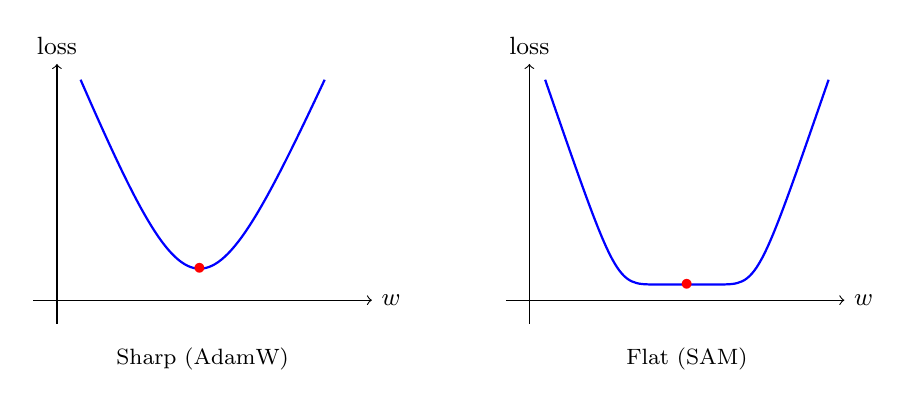
\begin{tikzpicture}[font=\small]
  \draw[->] (-0.3,0) -- (4.0,0) node[right]{$w$};
  \draw[->] (0,-0.3) -- (0,3) node[above]{loss};
  \draw[thick,blue] (0.3,2.8) .. controls (1.7,-0.4) and (1.9,-0.4) .. (3.4,2.8);
  \node at (1.85,-0.75) {\footnotesize Sharp (AdamW)};
  \node[red] at (1.81,0.4) {$\bullet$};
  \begin{scope}[xshift=6cm]
    \draw[->] (-0.3,0) -- (4.0,0) node[right]{$w$};
    \draw[->] (0,-0.3) -- (0,3) node[above]{loss};
    \draw[thick,blue] (0.2,2.8) .. controls (1.1,0.2) .. (1.6,0.2)
                      -- (2.4,0.2) .. controls (2.9,0.2) .. (3.8,2.8);
    \node at (2.0,-0.75) {\footnotesize Flat (SAM)};
    \node[red] at (2.0,0.2) {$\bullet$};
  \end{scope}
\end{tikzpicture}
\caption{Loss landscape geometry \parencite{li2024revisitingcatastrophicforgettinglarge}. A small weight shift in a sharp valley (AdamW) triggers a large loss spike on prior tasks; in a flat valley (SAM) the same shift preserves low loss.}
\label{fig:loss_landscape}
\end{figure}

\subsection{The Role of Low-Rate Replay}
At the data level, Scialom et al. \parencite{scialom-etal-2022-fine} demonstrate that an ultra-low replay fraction (between $0.25\%$ and $1\%$ of historical data) is sufficient to preserve a model's general zero-shot ability at negligible compute overhead, as summarized in Table~\ref{tab:replay_ratio}. This makes replay an inexpensive stabilizer that this work adopts when adapting behavior via LoRA.

\begin{table}[H]
\centering
\small
\caption{Impact of replay ratio on zero-shot retention \parencite{scialom-etal-2022-fine}.}
\label{tab:replay_ratio}
\begin{tabularx}{\textwidth}{c c c c X}
\hline
\textbf{Replay \%} & \textbf{Target loss} & \textbf{Zero-shot Acc (\%)} & \textbf{Compute} & \textbf{Remark} \\
\hline
0.00 (naive) & 1.72 & 22.4 & 1.000$\times$ & complete catastrophic forgetting \\
0.25 & 1.78 & 48.6 & 1.0025$\times$ & partial recovery \\
0.50 & 1.82 & 53.4 & 1.005$\times$ & strong retention of general reasoning \\
1.00 & 1.87 & 54.8 & 1.010$\times$ & near pre-trained ceiling \\
5.00 & 1.95 & 55.1 & 1.050$\times$ & saturation; new-task learning slows \\
\hline
\end{tabularx}
\end{table}

\subsection{Benchmarks and the Fragility Hierarchy}
Standardized benchmarks quantify forgetting along complementary axes. TRACE \parencite{wang2023tracecomprehensivebenchmarkcontinual} measures degradation of general ability, instruction following, and safety ($\Delta R^{G}$, $\Delta R^{I}$, $\Delta R^{S}$) across eight tasks, while ConTinTin \parencite{yin-etal-2022-contintin} evaluates continual learning from task instructions and shows that tasks with overlapping label spaces induce the strongest forgetting. A consistent finding is a \emph{fragility hierarchy}: safety alignment is highly persistent, whereas multi-step reasoning is the most vulnerable to decay. The standard metrics are Overall Performance (OP), Backward Transfer (BWT), Forward Transfer (FWT), and the logit-based Forgetting Gradient (FG), which is more sensitive than ground-truth accuracy.

Finally, Table~\ref{tab:fg_lora} bridges to the next section by quantifying how parameter-isolation methods control forgetting: orthogonal LoRA (O-LoRA) reduces the Forgetting Gradient by roughly fortyfold relative to vanilla LoRA \parencite{repec:axf:aidtaa:v:3:y:2026:i:1:p:52-61}, motivating the parameter-efficient techniques surveyed in Section~\ref{sec:peft}.

\begin{table}[H]
\centering
\small
\caption{Forgetting Gradient (FG \%, lower is better) across PEFT configurations \parencite{repec:axf:aidtaa:v:3:y:2026:i:1:p:52-61}.}
\label{tab:fg_lora}
\begin{tabularx}{\textwidth}{X c c c}
\hline
\textbf{Setup} & \textbf{Domain FG\%} & \textbf{Reasoning FG\%} & \textbf{Reading FG\%} \\
\hline
Full fine-tuning & 42.45 & 37.90 & 42.29 \\
LoRA ($r{=}64$) & 40.43 & 40.73 & 43.66 \\
LoRA ($r{=}128$) & 42.71 & 40.90 & 44.95 \\
Prefix-tuning & 37.15 & 38.54 & 42.05 \\
O-LoRA ($r{=}64$, $\lambda{=}0.5$) & 1.11 & 0.43 & $-1.20$ \\
O-LoRA ($r{=}128$, $\lambda{=}0.5$) & 0.77 & 0.25 & $-0.24$ \\
\hline
\end{tabularx}
\end{table}

In summary, catastrophic forgetting is a structural property of parametric adaptation rather than a tunable artifact. This reinforces the strategy of freezing the backbone and offloading volatile legal facts to retrieval, while reserving lightweight, isolation-based parameter updates for behavioral adaptation.
